\chapter{Analysis \& System Design}

\section{Changes to Current Control System}
\label{sec:Control_System}
This project is based on the system that is currently use. It controls PTU and takes readings from the inclinometer. Current system consists of the Gumstix minicomputer, GPIO14 chip, relays, inclinometer, PTU, server side code (running on Gumstix), client side code (provides API for the interaction with the main system) and the library implementing PTU TASS communication protocol to interact with the PTU.

There was a decision made by the client to replace the platform (Gumstix) that is currently used. The rationale behind the decision were client's concerns about the currently used Gumstix computer which is getting old. In case of a breakdown it would be difficult to find the replacement parts. One of the features requested was the ability to compile accompanying code on the platform itself (this is currently impossible on the Gumstix due to the hardware limitations) instead of cross-compiling code on the PC and then uploading executables to the Gumstix. Following a thorough discussion Raspberry Pi minicomputer was chosen as a replacement platform. It has enough power to compile the code as well as all the required interfaces for the connection of the other equipment. PTU TASS library will be reused and its functionality extended to implement the new features. Server and client side codes will be adjusted to provide access to the new functionality.

\section{System Architecture Overview}
As mentioned in the ~\ref{sec:Control_System} section, there will be both hardware and software parts in this project, they will be discussed further in this chapter. The server side will consist from the software running on the Raspberry PI minicomputer and handling all client requests. Connection will be initiated by the client over the TCP/IP protocol. Client side application will be using provided AberBox API to send/receive commands. Overall system architecture is presented on the figure ~\ref{fig:SystemArchitectureOverview}

\begin{figure}[H]
\centering
\centerline{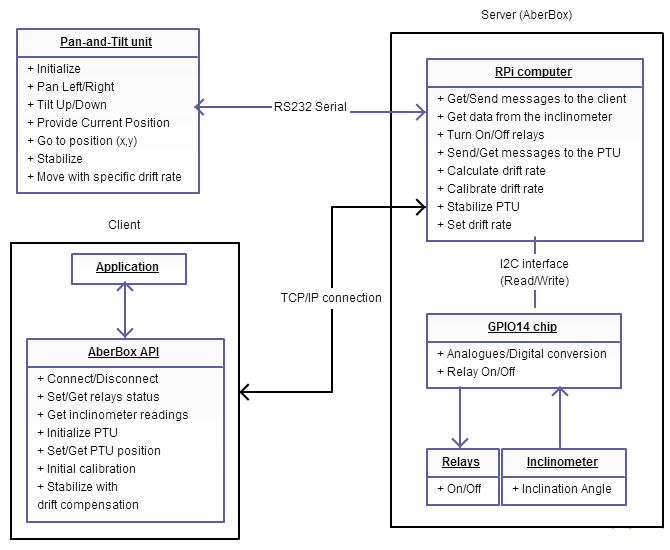
\includegraphics[scale=0.80]{./images/SystemArchitectureOverview}}
\caption{System Architecture Overview}
\label{fig:SystemArchitectureOverview}
\end{figure}

\section{Hardware Design}
The proposed system will consist of the Raspberry Pi minicomputer(RPi), analogue inclinometer, GPIO14 chip, relays and the PTU.

\subsection{RPi}
As a platform for the main control system Raspberry Pi minicomputer was chosen. It will replace the currently employed for this task Gumstix single board computer which provides limited control over the PTU. 

RPi is a credit-card-sized single-board computer with a 512 MiB of RAM and 700 MHz ARM based CPU. It is powerful enough for the proposed tasks to be completed and have all the required interfaces to be connected to the other peripheral. It has GPIO pins, including SPI and I$^2$C interfaces, UART serial console, 5v and GND supply pins. Such a powerful device may be an overkill for this task, but the decision was made by the client. Furthermore in the future it can be used to handle additional tasks.

\subsection{Inclinometer}
An inclinometer will be used to get data about the current chassis position in the space. The client suggested to use the SCA121T dual axis inclinometer (figure~\ref{fig:SCA121T-D05_inclinometer}) bolted to the chassis of the rover. It will provide the information about the inclination angles during PTU drift rate calibration. We will need a A/D converter, since it is a analogue device.

\begin{figure}[H]
\centering
\centerline{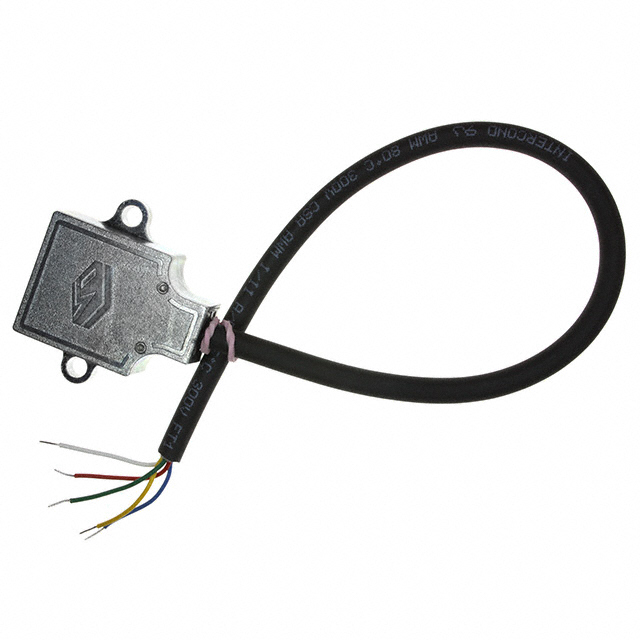
\includegraphics[scale=0.20]{./images/SCA121T}}
\caption{SCA121T-D05 Inclinometer}
\label{fig:SCA121T-D05_inclinometer}
\end{figure}

\subsection{GPIO14 Chip}
The GPIO14 chip is a pre-programmed PIC16F818 micro controller. It intends to provide general purpose I/O expansion on the $I^2$C bus. It has 14 general purpose I/O lines and 5 analogues input channels with 10-bit A/D conversion \cite{GPIO14}. GPIO14 chip will be used to convert inclinometer signal from the analogue format to digital and to switch on/off relays. This chip will be connected over the I$^2$C bus to the RPi.

\subsection{PTU}
Pan-and-Tilt Unit is a high-precision integrated motion control systems produced by the Sagebrush Technology (now part of the RIEtech Global, LLC \cite{RIEtech_Global}). It is designed for the <10Kg payloads and is often used to hold cameras, antennas or for instrument positioning. To connect it to the RPi (which has TTL interface) RS-232 to TTL converter was used. As a part of this project it is used to hold a panoramic camera. 

\section{Software Design}
This study will be based on the code that is already used on the Gumstix. It is currently used to send control commands to the PTU, get readings from the inclinometer and switch on/off relays. The code base consists of three main parts: the client side software, the server side software (running on the Gumstix and responding to client calls) and the library that implements PTU TASS communication protocol. 

\subsection{TASS library}
TASS library implements the protocol to communicate with the PTU. All communication is done over the serial interface.  The library implements basic commands, including pan left/right, tilt up/down, get/set position, get/set rotation limits.

One of the objectives of this project is to add implementation for the 'stabilize' and 'drift rate' commands as well as logic for the drift rate calculation.

\subsection{Server Side}
The server side software is responsible for the overall control of the PTU and inclinometer. It will be running on Raspberry Pi minicomputer and will respond to the client commands. On of the main challenges is to port the current system from the Gumstix to the RPi platform and make it work.

\subsection{Clint Side}
The client side software provides an API to interact with the server Side. The connection is made over the TCP/IP protocol. The plan is to extend the API upon the creation of the new stabilization functionality. 

\subsection{Operating System}
Raspbian is a free operating system that will be running on the RPi. It requires some initial configuration before the main software can be successfully run. Firstly, it requires configuration to prevent Linux from using the serial port; it also needs WiringPi library \cite{WiringPi} installed to successfully communicate over the I$^2$C bus with the GPIO14 chip. All the necessary configuration is covered in Appendix A.  